\chapter{Related Work and State of the Art}
\label{chap:related_work}

\section{Selection rule and exclusion of review papers}

This chapter focuses on original research papers, prototypes, experimental systems, and case studies. Review papers, overview papers, bibliometric papers, systematic reviews, and student theses are excluded from the main evidence base. They may help identify terminology or additional papers, but they are not used here as primary sources for definitions, figures, or the comparative synthesis.

The selected papers cover IoT-based irrigation and monitoring, machine-learning-based irrigation decision support, Digital Twin scheduling systems, reinforcement learning, interoperability, and crop water-stress Digital Twins. The objective is to compare concrete systems rather than to summarize broad survey classifications.

\section{IoT-based smart irrigation and monitoring systems}

Kodali and Sarjerao propose a low-cost irrigation system using a soil moisture sensor, an ESP8266 NodeMCU-12E, MQTT communication, web/mobile observation, and pump status reporting \cite{kodali2017mqttirrigation}. Its architecture is simple and reproducible: a field sensor provides the irrigation variable, the controller handles connectivity and actuation, and MQTT transfers messages between the device side and the monitoring side. The validation is a prototype demonstration. Its main limitation is that it does not maintain a synchronized virtual state or Digital Twin history.

Architecturally, the paper uses the soil-moisture sensor as the main data source, the ESP8266 NodeMCU-12E as both controller and connectivity node, MQTT/Thinger.io as the broker and monitoring platform, and a relay-pump loop for local actuation. Data and pump state are displayed through web and mobile views, while the control logic remains limited to the moisture/pump status loop. This makes the paper relevant for Agrio's MQTT and low-cost actuation background, but it does not include a Digital Twin state, what-if simulation, agronomic validation workflow, or traceable recommendation layer.

\begin{figure}[H]
    \centering
    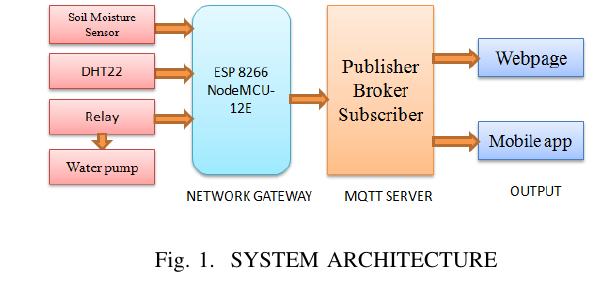
\includegraphics[width=0.72\textwidth]{figures/research_papers/kodali_original_architecture_figure.png}
    \caption{MQTT-based smart irrigation architecture proposed by Kodali and Sarjerao. Reproduced from Kodali and Sarjerao~\cite{kodali2017mqttirrigation}.}
    \label{fig:kodali_mqtt_irrigation_architecture}
\end{figure}

Balaceanu et al. present a Libelium-based IoT monitoring solution for precision agriculture \cite{balaceanu2019libelium}. The work is important because it uses a multi-variable sensing approach instead of relying only on soil moisture. The monitored variables include agricultural and atmospheric measurements useful for understanding irrigation context. The study focuses on monitoring and database construction, so prediction, simulation, recommendation, and physical actuation remain outside its main contribution.

The Libelium system is organized around agricultural sensing nodes, a Meshlium gateway, local persistence, and visualization. The paper reports monitoring of air temperature, relative humidity, soil humidity, atmospheric pressure, and solar radiation, with Meshlium parsing and storing data in a database before visualization. This architecture is useful for Agrio because it shows why irrigation decisions should consider more than a single moisture value. Its limitation is that it remains a monitoring and data-collection system: it does not implement prediction, simulation, user validation, or pump-control execution.

\begin{figure}[H]
    \centering
    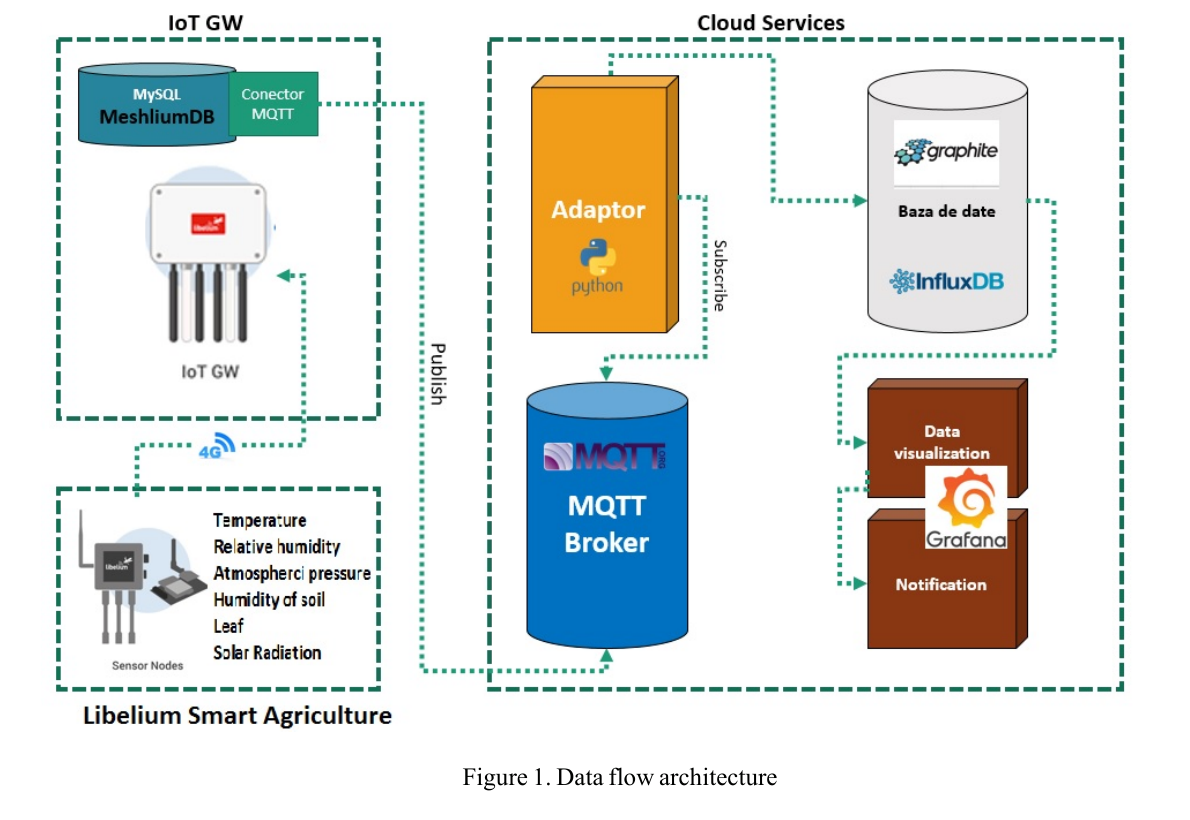
\includegraphics[width=0.95\textwidth]{figures/research_papers/balaceanu_original_libelium_architecture_figure.png}
    \caption{Libelium-based precision-agriculture monitoring architecture proposed by Balaceanu et al. Reproduced from Balaceanu et al.~\cite{balaceanu2019libelium}.}
    \label{fig:balaceanu_libelium_monitoring_architecture}
\end{figure}

Gupta et al. propose an IoT-enabled automated irrigation system for water and energy efficiency using soil moisture, temperature, and humidity sensing connected to an Arduino-based controller \cite{gupta2025iotirrigation}. The system includes automated control and mobile monitoring. Its relevance is the connection between sensing, automation, and resource efficiency. Its limitation for this thesis is the absence of an explicit Digital Twin state, what-if simulation layer, and traceable recommendation workflow.

\section{Machine-learning-based irrigation decision support}

Tancredi et al. study a Digital Twin enhanced with machine-learning algorithms for irrigation management using sensor data \cite{tancredi2025irrigationdt}. The paper is directly relevant because it treats irrigation management as a data-driven classification problem and connects ML to a Digital Twin direction. Its inputs are sensor-derived data, its objective is irrigation decision support, and its validation is based on algorithmic evaluation. Figure~\ref{fig:tancredi-ml-dt-irrigation} is reproduced from this paper.

Ed-Daoudi et al. present predictive irrigation as an integrated approach using IoT sensors, machine-learning algorithms, and adaptive scheduling \cite{eddaoudi2024predictiveirrigation}. The paper is useful because it frames predictive irrigation as a bridge between monitoring and intelligent scheduling. Its limitation is that it provides less detail about synchronized Digital Twin state management and the full measurement-to-actuation trace required by this thesis.

\section{Digital Twin irrigation scheduling systems}

Bellvert et al. assimilate Sentinel-2 biophysical variables into a Digital Twin for automated vineyard irrigation scheduling \cite{bellvert2023vineyarddt}. Their system combines remote sensing, local information, water-balance logic, and scheduling parameters to support regulated deficit irrigation. The work is valuable because it is field-oriented and directly addresses irrigation scheduling. Its limitation for the present prototype is the need for vineyard-specific calibration, remote-sensing inputs, and field-scale validation.

Millan et al. evaluate the Irri\_DesK Digital Twin in a 15-hectare commercial processing tomato farm \cite{millan2025tomatodt}. The system integrates plot information, soil moisture sensors, climate data, simulation models, and irrigation outputs to adjust irrigation doses. This study is especially important because it reports field-scale validation and compares Digital Twin-based management with conventional farmer management. Figure~\ref{fig:millan-tomato-dt-workflow} shows the data and simulation workflow.

\begin{figure}[H]
    \centering
    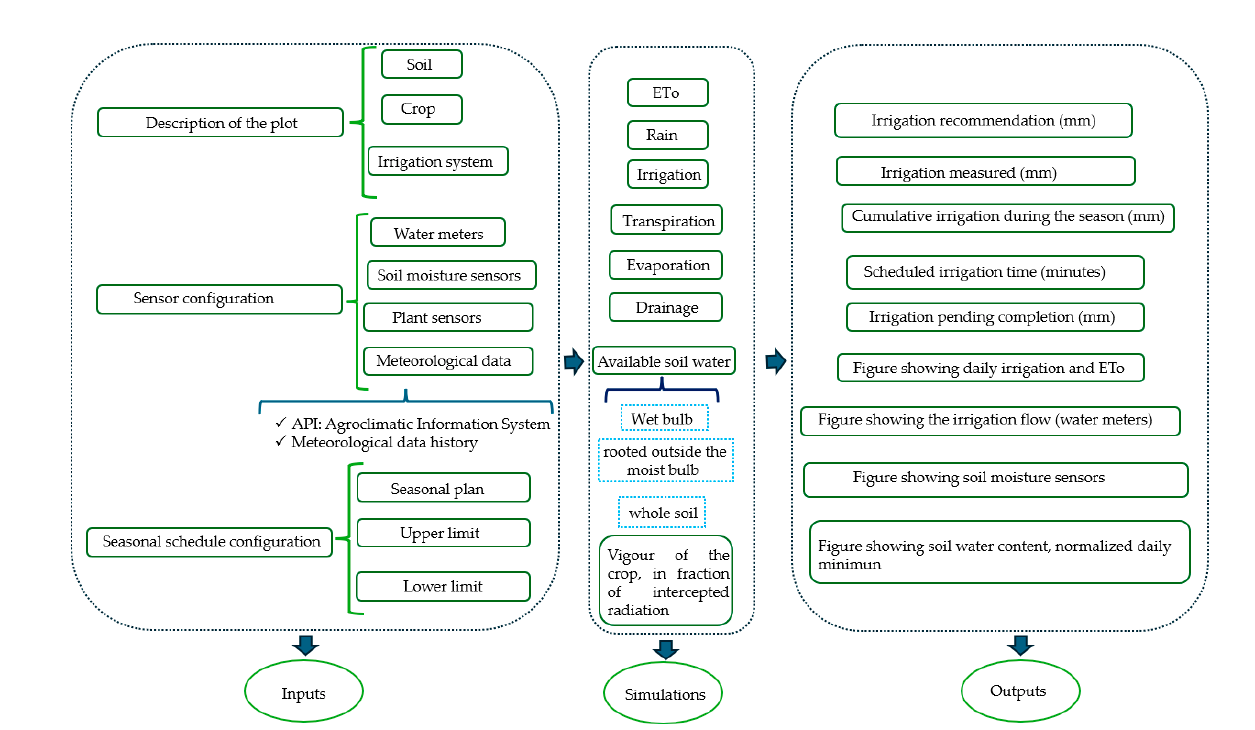
\includegraphics[width=0.9\textwidth]{figures/research_papers/millan_tomato_dt.png}
    \caption{Digital Twin workflow for water-efficient irrigation management in a processing tomato farm. Reproduced from Millan et al.~\cite{millan2025tomatodt}.}
    \label{fig:millan-tomato-dt-workflow}
\end{figure}

\section{Reinforcement learning, interoperability, and crop water-stress Digital Twins}

El Hachimi et al. propose a framework combining Digital Twins and deep reinforcement learning for collective irrigation water distribution systems \cite{elhachimi2025collectiveirrigationdt}. The study targets open-channel irrigation systems and uses an irrigated area in the Tensift basin in Morocco as a case study. It is useful for future work because it moves beyond single-zone scheduling toward coordinated distribution in shared infrastructure.

The architecture couples an R3 irrigation-district Digital Twin with a deep deterministic policy gradient agent. The Digital Twin represents crop-growth and open-channel network behavior over full-season simulations, while the agent learns policy recommendations from simulated interactions. Evaluation is based on yield, seasonal irrigation, and water-use efficiency indicators. For this thesis, the paper provides a reference for future optimization, but it should not be presented as implemented in Agrio: the current prototype uses Random Forest inference, what-if simulation, supervised recommendation, and human validation rather than reinforcement-learning control.

\begin{figure}[H]
    \centering
    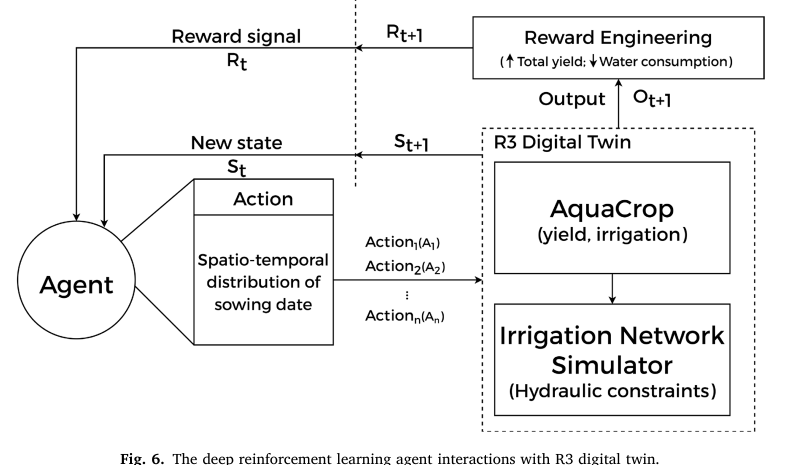
\includegraphics[width=0.95\textwidth]{figures/research_papers/elhachimi_fig6_dt_drl_framework.png}
    \caption{Deep reinforcement-learning agent interactions with the R3 Digital Twin. Reproduced from El Hachimi et al.~\cite{elhachimi2025collectiveirrigationdt}.}
    \label{fig:elhachimi_dt_drl_architecture}
\end{figure}

Kallenberg et al. introduce interoperable agricultural Digital Twins with reinforcement-learning intelligence \cite{kallenberg2025interoperabledt}. Their architecture augments agricultural models as Digital Twins, connects reinforcement-learning agents to decision recommendations, and uses a FIWARE-based interoperability layer. Although it is not limited to irrigation scheduling, it is relevant because future agricultural Digital Twins will need interoperability between models, context data, and AI services.

\begin{figure}[H]
    \centering
    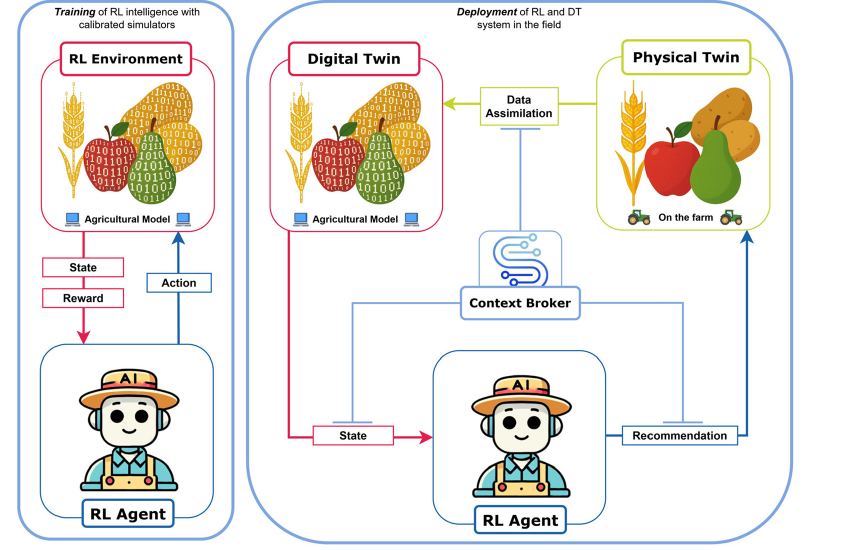
\includegraphics[width=0.95\textwidth]{figures/research_papers/kallenberg_fig1_interoperable_adt_architecture.png}
    \caption{Interoperable agricultural Digital Twin concept connecting calibrated models, reinforcement-learning agents, physical twins, and a context broker. Reproduced from Kallenberg et al.~\cite{kallenberg2025interoperabledt}.}
    \label{fig:kallenberg_interoperable_adt_architecture}
\end{figure}

Liu et al. develop a cotton canopy Digital Twin from a water-stress perspective \cite{liu2025cottondt}. Their framework includes a crop visualization module, a water-interaction module, and biomass-transfer rules. This work is relevant because it represents crop response under water stress rather than only irrigation infrastructure. Its limitation for this thesis is that it does not provide a direct pump-control or irrigation-actuation workflow.

\begin{figure}[H]
    \centering
    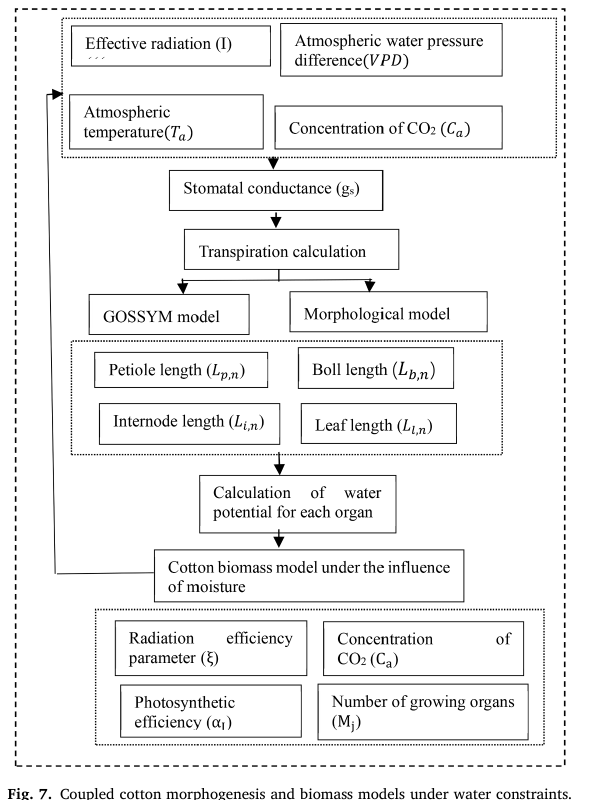
\includegraphics[width=0.70\textwidth]{figures/research_papers/liu_fig7_cotton_water_stress_dt_framework.png}
    \caption{Coupled cotton morphogenesis and biomass models under water constraints. Reproduced unchanged from Liu et al.~\cite{liu2025cottondt}.}
    \label{fig:liu_cotton_water_stress_dt_framework}
\end{figure}

\section{Comparative synthesis}

Table~\ref{tab:original-research-comparison} compares the retained original research papers according to their agricultural context, data sources, integration approach, model or AI component, Digital Twin function, actuation/control support, validation type, and main limitation.

\begin{landscape}
\begin{scriptsize}
\setlength{\tabcolsep}{2pt}
\renewcommand{\arraystretch}{1.15}
\begin{longtable}{@{}p{0.10\linewidth}p{0.105\linewidth}p{0.105\linewidth}p{0.115\linewidth}p{0.10\linewidth}p{0.115\linewidth}p{0.095\linewidth}p{0.095\linewidth}p{0.12\linewidth}@{}}
\caption{Comparison of original research papers used in the early chapters}
\label{tab:original-research-comparison}\\
\toprule
Paper & Agricultural context & Data sources & Communication / integration & AI or model used & Digital Twin function & Actuation / control & Validation type & Main limitation \\
\midrule
\endfirsthead
\toprule
Paper & Agricultural context & Data sources & Communication / integration & AI or model used & Digital Twin function & Actuation / control & Validation type & Main limitation \\
\midrule
\endhead
Kodali and Sarjerao \cite{kodali2017mqttirrigation} & Small-scale smart irrigation & Soil moisture and pump status & ESP8266 NodeMCU and MQTT & Threshold/status logic & None; IoT control system & Pump switching & Prototype demonstration & No Digital Twin or field-scale agronomic validation \\
Balaceanu et al. \cite{balaceanu2019libelium} & Precision-agriculture monitoring & Temperature, soil humidity, pressure, solar radiation & Libelium IoT monitoring platform & None & None; monitoring database & No direct irrigation control & Monitoring experiment & Monitoring focus without prediction or simulation \\
Tancredi et al. \cite{tancredi2025irrigationdt} & Sensor-data irrigation management & Sensor dataset & Digital Twin and ML workflow & ML classification algorithms & ML-enhanced decision support & Decision support for irrigation status & Algorithm evaluation & Field and implementation detail limited \\
Bellvert et al. \cite{bellvert2023vineyarddt} & Commercial vineyard & Sentinel-2 biophysical variables and local data & Digital Twin and IoT-enabled scheduling application & Water-balance simulation and data assimilation & Automated irrigation scheduling & Scheduling recommendations & Commercial vineyard case & Specialized remote-sensing and calibration requirements \\
Millan et al. \cite{millan2025tomatodt} & Processing tomato farm & Soil moisture, climate data, simulation inputs & Irri\_DesK Digital Twin workflow & Soil-water-balance simulation & Daily dose adjustment and scheduling & Irrigation strategy management & 15 ha commercial farm evaluation & Crop- and site-specific calibration required \\
El Hachimi et al. \cite{elhachimi2025collectiveirrigationdt} & Collective open-channel irrigation & Canal and irrigation-system state data & Digital Twin simulation framework & Deep reinforcement learning & Optimization environment for water distribution & Policy recommendations for distribution & Case-study simulation in Morocco & Advanced setup; operational deployment remains future work \\
Kallenberg et al. \cite{kallenberg2025interoperabledt} & Interoperable smart farming & Field data and model context entities & FIWARE-based interoperability layer & Reinforcement learning agents & Model-based Digital Twins connected to AI agents & Recommendations for agricultural operations & Architecture and operational demonstration & Not specific to irrigation scheduling \\
Ed-Daoudi et al. \cite{eddaoudi2024predictiveirrigation} & Sustainable cultivation and irrigation & IoT sensor data & Integrated predictive-irrigation system & Machine-learning models & Not a full Digital Twin & Adaptive scheduling support & Case-study-oriented evaluation & Limited Digital Twin synchronization and actuation detail \\
Gupta et al. \cite{gupta2025iotirrigation} & Automated irrigation for water and energy efficiency & Soil moisture, temperature, humidity & Arduino-based IoT system and mobile monitoring & Predictive irrigation algorithm & None; IoT automation & Automated irrigation control & Field-trial evaluation & No Digital Twin simulation layer \\
Liu et al. \cite{liu2025cottondt} & Cotton canopy under water stress & Crop and water-stress variables & Crop Digital Twin framework & Water-interaction and biomass-transfer modules & Crop-growth and water-stress simulation & No direct irrigation actuation & Methodological case study & Irrigation control is indirect \\
\bottomrule
\end{longtable}
\end{scriptsize}
\end{landscape}

The synthesis shows that no single paper covers the whole scope required by the thesis. Low-cost MQTT systems are practical but limited to monitoring and control. Digital Twin scheduling systems are stronger agronomically but require field-scale calibration. ML systems provide prediction but must be integrated into a complete cyber-physical workflow. Reinforcement-learning and interoperability works point toward future extensions rather than immediate prototype requirements.

\section{Summary}

This chapter reviewed original research papers only and separated them from review or orientation sources. The related work shows an integration gap between low-cost IoT control systems and field-validated Digital Twin irrigation systems. This observation motivates the scientific positioning and comparative analysis developed in Chapter~\ref{chap:scientific_positioning}.
